% ============================================================================
% DHG508 Final Design Paper & Post-Mortem
% Liu Runze (刘润泽) · 3140631 · Lingnan University
%
% Compile: XeLaTeX -> Biber -> XeLaTeX -> XeLaTeX
% On Overleaf: Menu -> Compiler -> XeLaTeX -> Recompile
% ============================================================================

\documentclass[12pt,a4paper]{article}

\usepackage{fontspec}
\newcommand{\MainLatinFont}{Times New Roman}
\newcommand{\FallbackLatinFont}{TeX Gyre Termes}
\newcommand{\MainCJKFont}{Noto Serif CJK SC}
\newcommand{\FallbackCJKFont}{FandolSong-Regular.otf}

\IfFontExistsTF{\MainLatinFont}
  {\setmainfont{\MainLatinFont}}
  {\setmainfont{\FallbackLatinFont}}

\usepackage{xeCJK}
\IfFontExistsTF{\MainCJKFont}
  {\setCJKmainfont{\MainCJKFont}}
  {\IfFontExistsTF{Songti SC}
    {\setCJKmainfont{Songti SC}}
    {\IfFontExistsTF{SimSun}
      {\setCJKmainfont{SimSun}}
      {\setCJKmainfont{\FallbackCJKFont}}}}

\usepackage[a4paper, margin=1in]{geometry}
\usepackage{setspace}
\usepackage{booktabs}
\usepackage{array}
\usepackage{graphicx}
\usepackage{csquotes}

% Chicago Manual of Style 18th ed., Notes-Bibliography (BibLaTeX + Biber)
\usepackage[notes, backend=biber, autolang=other, isbn=false]{biblatex-chicago}
\addbibresource{references.bib}

\renewcommand{\footnotesize}{\fontsize{10}{12}\selectfont}
\usepackage[hidelinks]{hyperref}

\title{\textbf{OBSERVATION LOG: A Duty Log You Have to Sign}\\[0.3em]
\large Design Rationale, Evidence Boundaries, and Post-Mortem}
\author{Liu Runze 刘润泽 (3140631)\\Lingnan University $\cdot$ DHG508 Critical Digital History\\
\small Live build: \url{https://observation-log-9t9.pages.dev}\\
\small Repository: \url{https://github.com/Luciaris7/dhg508-workspace}}
\date{25 November 2026}

\begin{document}
\maketitle

\begin{abstract}
\noindent
This paper asks how a bureaucratic record, not a monster, can carry a horror
game. \emph{OBSERVATION LOG} puts the player behind a duty log for seven nights:
you aim an antenna, sound the lake, plot an object that should not be on the
star chart, and submit a report on whether the image is anomalous. The question
is cultural rather than archival. No historical station is reconstructed here;
what is borrowed from history is the form of the record and the discipline it
imposes. The paper separates what is documented (\emph{据}) from what is inferred
(\emph{推断}) and invented (\emph{设}), shows which scholarly work justifies which
mechanic, and reports what the tests can and cannot prove.
\end{abstract}

\onehalfspacing

\section{Historical Question and Medium}

My question is what happens to authority when a record has no reader who can
verify it. A duty log compresses a world into entries: time, instrument, reading,
signature. Its authority is disciplinary rather than evidential. Nobody checks
the keeper's log against the lake; they check that the keeper filled it in. So a
log is a peculiar kind of document: it is at once the most trustworthy account of
a place and the only account, and the two are not the same thing. What kind of
horror becomes possible when the thing being recorded is the sole evidence that
it exists?

An essay can describe that position. It cannot put a reader in it. The design
claim of \emph{OBSERVATION LOG} is that only an interactive medium can make the
player perform the labour that produces the dread, and then show the record
turning against the person who signed it. The player does the work: four
recurring tasks, seven times. The report asks a single question, whether the day's
image shows an anomaly, and accepts one answer. From the sixth night the station
accepts only \emph{No}; a \emph{Yes} is thanked, re-read, and rewritten. The horror
is not that the player failed to see something. It is that the player saw it,
wrote it down, and filed it.

I should be exact about what is historical here. Birch Lake, Site 7, the
thirteen-year cycle and the blood-red aurora are invented; the historical material
is the \emph{form} — the duty log, the period desktop with its self-test strings,
the report that outranks the observer. The game therefore makes no claim about any
real station, and this paper makes none either.

\section{Sources and Scholarly Conversation}

\paragraph{Primary sources and their limits.}
The project has no archival primary source, and I will not pretend otherwise. The
closest thing to a document is the in-game work manual, which I wrote. What I do
have is seven games that supplied the mechanics: \emph{Iron Lung},
\emph{I Have No Mouth, and I Must Scream}, \emph{Fears to Fathom},
\emph{Firewatch}, the Chilla's Art series, \emph{Sally Face} and
\emph{Silent Hill}.\autocite{ironlung2022,ihavenomouth1995,fearstofathom2021,firewatch2016,chillasart2018,sallyface2016,silenthill1999}
They are cultural sources rather than evidence: they are where the mechanics come
from, not what the world was. This has a consequence I have to state plainly: the
\emph{据} tier in my evidence table is thin and is about form, not events. It
covers the ephemeris, the Morse alphabet, the period interface and the bilingual
copy. Everything about the station's meaning is \emph{推断} or \emph{设}.

\paragraph{Threat simulation, and the fear of not being able to see.}
Kjeldgaard-Christiansen and Clasen argue that horror games invite players to
simulate prototypical fear scenarios of uncertainty and danger.\autocite[2]{kjeldgaard2019threat}
They explain our fear of the dark as a fear of information poverty: darkness
limits access to information about the surroundings, which is precisely what lets
a threat approach unnoticed.\autocite[4]{kjeldgaard2019threat} They then describe
the genre as organised around threat assessment and threat negotiation, and its
appeal as a safe experience with prototypical fear
scenarios.\autocite[11]{kjeldgaard2019threat} This is the argument behind mechanic
one. In \emph{Iron Lung} the player photographs the outside world through a bad
camera;\autocite{ironlung2022} in my game the camera becomes a star chart, and the
anomaly is never drawn in the sky. It exists only as a circle whose diameter grows
from six pixels to one hundred and sixty across seven nights. The player is still
observing, but the object of observation is a figure that changes between
evenings, so the fear comes from comparison rather than from an event. Their point
also supplies my boundary: a safe frame is what makes the simulation bearable, and
if the frame is too safe the mechanic produces only tedium.

\paragraph{Uncanny bodies, and what low fidelity does.}
Tinwell, Grimshaw and Williams measured how perceived uncanniness varies with a
virtual character's human-likeness, and found that motion and sound exaggerate the
uncanny effect and the perceived frightfulness; characters rated as the least
synchronised were perceived to be the most frightening.\autocite[1]{tinwell2010uncanny}
I used this for the fifth mechanic. The world renders at 320 by 180 pixels in a
32-colour palette, so every figure is a silhouette, and the sixth mechanic's
intruder moves on a frame cycle that does not match its footstep sound. Low
fidelity is not an aesthetic preference here; it forces the player to complete the
body. My limit is obvious: their subjects judged humanoid characters on a rating
scale, and my intruder is a twelve-frame silhouette nobody has rated.

\paragraph{The gothic past, returning as a record.}
Kirkland examines how the gothic tradition operates inside survival horror, and
identifies four concerns: the intrusion of an eerie otherworld, a fragmented
narrative form, the sense of the past intruding on the present, and a
psychoanalytic dimension.\autocite[106]{kirkland2012gothic} That list maps onto
mechanics three and six more closely than any design advice could. My thirteen-year
cycle is the past intruding on the present in the most literal way available: the
archive lists only the three previous keepers, and the fourth is the player. The
fragmented form becomes a document that rewrites itself after submission, which is
my answer to a problem Kirkland raises but does not solve for a game designer: a
fragmented narrative usually fragments the plot, and I wanted the fragmentation to
sit inside an object the player trusts.

\paragraph{The gap I am working in.}
Taken together these three works explain why uncertainty is tolerable in a safe
frame, how a low-fidelity body becomes frightening, and how a gothic past returns
in playable form. None of them is about paperwork. The contribution I claim is
narrow: to move the site of horror from the thing seen to the act of recording
it, and to make the player's compliance, not their courage, the variable that
decides the ending.

\section{Architecture and Boundaries}

\paragraph{Data and logic.}
There is no server, no account and no network call at runtime. Astronomical data
is precomputed and shipped: a truncated VSOP87 series for the planets (20 KB of
JSON), one lunar longitude and distance sample per day from 1980 to 2120 (412 KB
of binary), and a table of thirty-six reference dates used by the accuracy test.
GDScript evaluates the series at the player's calendar date, so the sky in the star
chart is the real sky of the evening they play. Story state is one small JSON file
in the browser's IndexedDB; a single decision function decides the ending.

\paragraph{Rendering.}
Every view is its own sub-viewport so that the pixel art and the shaders never
disagree about resolution: the world at 320 by 180 doubled to 640 by 360, the
simulated desktop at 640 by 360 with a CRT shader, and a post-processing shader
that quantises everything to the 32-colour palette with ordered dithering. The
menu layer is deliberately outside that stack and is never distorted.

\paragraph{Route to the public URL.}
Godot 4.7.2 exports a web build with threading disabled; the engine binary is 37.7
MB, which exceeds the 25 MiB per-file ceiling on Cloudflare Pages. The build
therefore ships a 9.7 MB gzipped engine plus a worker that inflates it with
\texttt{Decompression\allowbreak Stream} and serves it as
\texttt{application/\allowbreak wasm}. Figure~\ref{fig:schematic} shows the whole
path from generated assets to the live URL.

\begin{figure}[htbp]
  \centering
  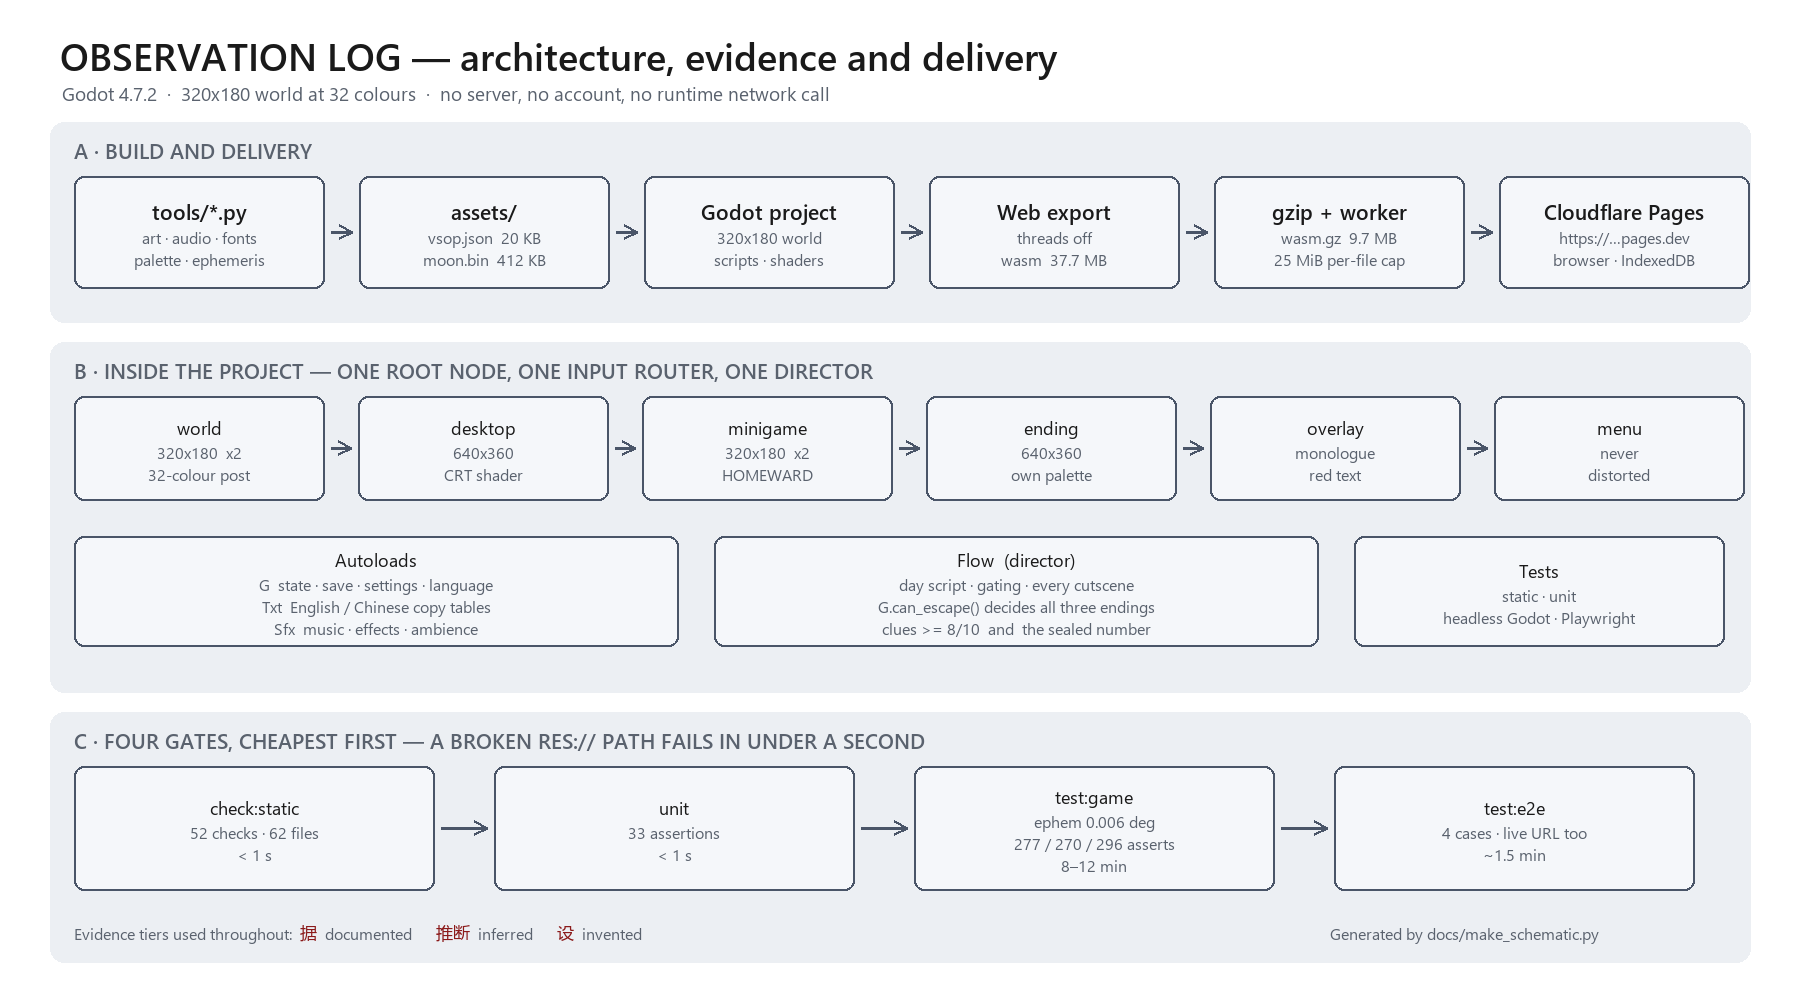
\includegraphics[width=0.62\textwidth]{schematic.png}
  \caption{From generated assets to the public URL, with the four test gates.}
  \label{fig:schematic}
\end{figure}

\paragraph{Temporal and epistemic cutoffs.}
The in-game calendar is not fixed. The first day is the real date of first play,
and the three earlier cycles are computed as thirteen, twenty-six and thirty-nine
years before it; the sealed record's Morse number is derived from those dates
rather than written into the code. The fiction is therefore anchored to the
player's calendar, which is also its limit: the game cannot represent a
historical 1999 because it is always happening now. The epistemic cutoffs are
stricter. The game never states the legend as fact, only as rumour on a
noticeboard and in a voicemail; the archive lists three prior keepers and
explains nothing; and the flesh god, the submerged church and all three endings
are invention, marked as such in the table that follows.

\section{Evidence Table}

Table~\ref{tab:evidence} is generated from \texttt{paper/evidence.csv} by
\texttt{make\_evidence\_table.py}; the LaTeX rows are never typed by hand. Each
row names the file that would falsify it.

\begin{table}[htbp]
  \centering
  \scriptsize
  \singlespacing
  \renewcommand{\arraystretch}{1.0}
  % Auto-generated from evidence.csv by make_evidence_table.py — edit the CSV, not this file.
\begin{tabular}{>{\raggedright\arraybackslash}p{0.21\textwidth}>{\raggedright\arraybackslash}p{0.16\textwidth}>{\raggedright\arraybackslash}p{0.22\textwidth}>{\raggedright\arraybackslash}p{0.06\textwidth}>{\raggedright\arraybackslash}p{0.21\textwidth}}
  \toprule
  \textbf{Claim / Element} & \textbf{Source / File} & \textbf{Locator} & \textbf{Level} & \textbf{Boundary / Limit} \\
  \midrule
  Star chart uses the real sky of the play date & Astronomy Engine VSOP87, precomputed & tools/ephem\_export.py; tests/ephem\_test.tscn & 据 & 0.006 deg vs a 0.1 deg threshold; says nothing about the fiction \\
  Radio codes are real Morse of a derived number & 4-2-2-4 grouping of twelve digits & g.gd; flow.gd; tests/ending\_test.gd & 据 & Real alphabet; the number it encodes is invented \\
  Desktop belongs to a 2001-2006 PC & Reconstruction from period screenshots & desktop.gd; plan.md sec.5 & 据 & No preserved machine consulted \\
  Duty log: antenna, sounding, chart, report & Composite of a remote post's routine & MYSTERY\_BIBLE.md sec.2 & 推断 & No single station documented \\
  Blood aurora is only ever a rumour & Noticeboard and prologue voicemail & txt.gd key rumor & 推断 & Deliberately unverifiable in the fiction \\
  Darkness is fear of missing information (mechanic 1) & Scholarly argument justifying the design & Kjeldgaard-Christiansen and Clasen, preprint p. 4 & 推断 & Explains why it should work; not that it does \\
  Desynchrony sharpens the uncanny (mechanic 5) & Scholarly argument justifying the design & Tinwell et al., accepted MS p. 1 & 推断 & Their subjects judged humanoids, not silhouettes \\
  Report coerces its own answer: Yes becomes No & Coercion branch in the director & flow.gd; tests/ending\_test.gd & 设 & Design fiction, not a historical claim \\
  Flesh god, submerged church, all three endings & Canon document & MYSTERY\_BIBLE.md sec.2 and sec.6 & 设 & No referent; guarded by consistency tests only \\
  Good ending needs the sealed number and 8 of 10 clues & Single decision function & g.gd lines 235-236 & 设 & One document still says 10/10; the code says 8/10 \\
  \bottomrule
\end{tabular}

  \caption{Claims and design elements with locators, evidence tiers
  (\emph{据} documented, \emph{推断} inferred, \emph{设} invented), and limits.}
  \label{tab:evidence}
\end{table}

\section{Verification and Playtesting}

\paragraph{What the four gates check.}
The gates are layered so that the cheapest failure happens first. A static check
over 62 source files validates \texttt{res://} references, JSON, the web export
preset and accidental leaks of local paths and keys; re-running it on 24 November
2026 gives 52 of 52 checks passing. A unit layer of 33 assertions covers the canon
constants, bilingual key parity, the audio bus layout and the contents of the
build directory. A headless Godot layer of roughly eight to twelve minutes runs the
ephemeris against the thirty-six reference dates (maximum error 0.006 degrees
against a 0.1 degree threshold), three complete playthroughs that assert at every
beat (277, 270 and 296 assertions), a forced-walk regression over six frame
intervals, and the ending, menu and dream scenes. A Playwright layer runs four
cases against the built site and against the live URL: no console errors, no 404s,
a real WebAssembly module, and a phone-sized viewport without clipping; all four
passed against the deployed build on 25 November 2026.\autocite{obslog2026live}

\paragraph{Two testers outside the build.}
The build was written by AI agents; both testers below are outside it. Tester A
was a friend who played without knowing the setting and returned a written report
on 17 November 2026 with six concrete items; I relayed it into
\texttt{docs/plan.md}. Five of the six changed the build: a prompt to exit the
ridge view, rewritten text in the boat-dock locker and in the sealed record, the
archive cut from an open list to exactly three prior cycles (1987, 2000, 2013) with
the Morse number re-derived, and the bed made usable on any night, which opened
the UFO ending. The date change is the one I can guard mechanically: the number is
now computed, so \texttt{tests/ending\_test.gd} fails if a constant is ever
hardcoded back in. Tester B was the commissioning player, whose 24-item report of
16 November 2026 reversed the central mechanic: the station wants \emph{No}, and a
\emph{Yes} is rewritten, which is the opposite of what I had implemented. Tester B
also reported that the live build had no sound. The page-level analyser showed a
signal of 0.128 RMS while the operating system's audio meter showed 0.000, which
localised the fault to buses created at runtime that the browser's audio driver
never connected; the fix moves the bus layout into a static resource, and five
assertions in \texttt{tests/unit/audio.test.mjs} now pin the layout, the bus names
and the send relationships.

\paragraph{What the tests cannot do.}
Every gate above proves internal consistency: the clues do not drift, the
thresholds hold, both languages say the same thing, the ephemeris does not decay.
None of them measures whether the second night is frightening. The playthrough
assertions are the strongest evidence I have, and they are evidence about
correctness, not about effect.

\section{Post-Mortem}

\begin{enumerate}
  \item \textbf{What worked.} Three things earned their cost. The layered gate
  caught a broken resource path in under a second instead of after a twelve-minute
  playthrough. Generating every asset from a script meant a palette change
  regenerated the art, the fonts and the distortion typefaces together, with no
  hand-editing of images. And reducing the endings to one function,
  \texttt{G.can\_escape()}, meant the three routes could be asserted rather than
  described.

  \item \textbf{What failed.} The reporting arc was backwards for most of the
  build: I had the station demanding \emph{Yes}, which inverts the whole point,
  and no automated test could have caught it because the test only checked that
  some answer was accepted. Tester B found it on the first evening. The seventh
  night's forced walk could wedge forever, because position accumulated by speed
  and overshot its target; it is fixed with \texttt{move\_toward} and guarded by
  24 motion cases. Two smaller failures are worth naming because they were silent:
  a red-text call referenced a copy key that did not exist, and the lookup returned
  an empty string, so a door opened onto nothing; and the canon document still says
  the good ending needs all ten clues while the code requires eight, which is
  exactly the kind of drift a table cannot catch and a test can.

  \item \textbf{What changed.} The scope moved from three survey points with a
  5000-point key in the desktop game to two points and a 2000-point target,
  because a 5000-point threshold made the key unreachable and an unreachable clue
  is a bug wearing a mystery's clothes. The eyes came out of every scene and
  ending illustration. The antenna moved to a hilltop with a separate scene,
  because standing next to your own antenna was not plausible. And the god stopped
  being explained: what is deliberately left unknown is now wider than what is
  revealed.

  \item \textbf{Limits and AI tools.} A playthrough is forty to sixty minutes,
  there is one save slot, and the web build is keyboard-only, so a phone can see the
  game but not play it; the first load is about 38 MB. The second tester's material
  is one written report rather than a recorded session, which is thinner evidence
  than I would like. The build used Claude Opus 5.5, GLM 5.3 Flash, DeepSeek V4.1
  Flash and ChatGPT 6.1 Sol across different passes. The division of labour is the
  part worth recording: the AI wrote code and drafts quickly and consistently, and
  every design decision, every rejection and every line of canon came from the
  humans. Where the AI filled a gap itself, the gap is still listed in
  \texttt{docs/DESIGN.md} as pending review rather than quietly closed.
\end{enumerate}

\singlespacing
\small
\printbibliography[title={Bibliography}]

\end{document}
